\begin{song}{title=\predtitle\centering Pažitka \\\large Xavier Baumaxa  \vspace*{-0.3cm}}  %% sem se napíše jméno songu a autor
\begin{centerjustified}

\sloka
Krajina ^*{A}sv ádí k podzimním ^{C#mi{\color{white}\_}\:\,}výletům,

tripům do ^{F#mi}mládí a častým ^*{D}úl etům.

Barevný ^*{A}lis tí je rázem ^{C#mi{\color{white}\_}\:\:}pestřejší,

hlavu ^{\:\:\,F#mi\z}ti~čistí,~no~a ty jsi ^*{D}by střejší.


\refren
/: ^*{A}Pa šuješ zážitky,

^*{E}pa šuješ všechno co se ^{F#mi}dá,\:\:\:\:

\phantom{.}

sáčky suchý pažitky,

^{D{\color{white}\_}}tomu se říká dobrá nálada. :/



\sloka
Hladina tůní pomalu vychladá,

je konec vůním a léto uvadá.

Na stehna fenek, dopadl dlouhý stín,

skončil čas trenek, ale já zas něco vymyslím.


\refren


\sloka
Cenzura.


\refren

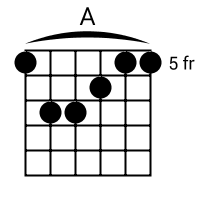
\includegraphics[width = 3cm]{../Akordy/a2verze.png}
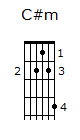
\includegraphics[width = 3cm]{../Akordy/cxm.png}
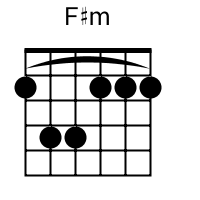
\includegraphics[width = 3cm]{../Akordy/fxm.png}


\end{centerjustified}
\setcounter{Slokočet}{0}
\end{song}
